% BEGIN SECTION 7
% Last updated by Milan Ilnyckyj 2013-08-26



		\singlespacing
		\section{Short answers to common questions}
		\label{sec:FAQ}
		\doublespacing
		


		% Has incorporated comments from Alena Prazak




	\subsection{Why should the university `take sides' in this matter? Is it appropriate for the university to take stances on social and political issues?}
	\label{TakeSides}



The University of Toronto's \nameref{PolicySocialPolitical} and \nameref{ProceduresResponding} establish appropriate criteria for deciding when an issue is no longer properly the subject of academic debate, meaning that divestment is justified.
For the reasons extensively elaborated in this brief, divestment from fossil fuel companies is compatible with this policy.
Furthermore, the university has already taken several actions that acknowledge the seriousness of climate change and the appropriateness of changing university practices in order to make it less severe.\footnote{See: \nameref{UofTActions}}



Divestment from fossil fuels follows the precedents established by the university in divesting from South Africa in response to apartheid and divesting from tobacco in response to the human health impacts.\footnote{See: \nameref{sec:LikeTobacco}}
The benefits from burning fossil fuels accrue to those who use them directly --- groups that are disproportionately influential politically and legally.
By contrast, the harms from burning these fuels are imposed on everybody, including those who have made little use of them historically and defenceless members of future generations.



% Note, some of the text in the following paragraph comes from the Executive Summary



Permitting unmitigated climate change challenges the core values of the university, including its ``resolute commitment to the principles of equal opportunity, equity and justice''.\footcite{InstitutionalPurpose}
If future generations are to have equal opportunities, they cannot inherit a planet that has been impoverished by uncontrolled climate change.
Similarly, the principles of equity and justice forbid us from ignoring what we know about the harms of greenhouse gas pollution by continuing to impose risk and suffering on innocent people around the world now and in future generations.



Fossil fuel divestment is also justified because governments have been ineffective in combatting climate change.
The \emph{United Nations Framework Convention on Climate Change} came into force in 1994, and there have already been 20 Conferences of the Parties.
The \emph{Kyoto Protocol} came into force in 2005.
Despite all this diplomacy and effort, greenhouse gas pollution continues to increase, and the amount of \ce{CO2} in the atmosphere continues to grow to ever-more-dangerous levels.
Organizations including universities and other institutional investors can play an important role in redirecting investment away from making the problem worse and toward solving it.
They can also help push governments to act more efficaciously and with greater speed.



In 1972, Yale University published \emph{The Ethical Investor: Universities and Corporate Responsibility}.
The book describes a ``moral minimum'' obligation.
It is not possible for universities to take action in response to every social wrong, but they should work to ``avoid and correct self­caused social injury''.\footcite[][p. 21]{EthicalInvestor}
Given the robustness of our current scientific understanding of climate change, investing in the further development and exploitation of fossil fuel resources falls into this category of behaviours.\footnote{\emph{The Ethical Investor} also describes the Key Gardens Principles of need, proximity, capability, and last resort. 
They require a social harm which calls for redress, proximity in the sense of having an understood effect, having an opportunity to act, and last resort. 
In discussing `last resort', the book explains that: ``the guilt of all becomes the guilt of no one. This result is unacceptable. We may not be able to avoid the world's guilt, but we can seek to reduce the level of injury'' (p. 26). 
The book also explains: ``if the university is able, by non self­sacrificial means, to mitigate injury caused by a company of which it is an owner, it would not seem unreasonable to ask it to do so'' (p. 24)}
The Terms of Reference of U of T's Responsible Investing Committee also recognize: ``that certain principles related to social, environmental or governance matters may be established to supplement our investment strategies without compromising our fiduciary obligations'', that ``[s]uch principles may in fact be both prudent and consistent with the University's academic mission'', and that ``it is widely acknowledged that, for a company to be financially successful in the long term, management must engage in sustainable and sound business practices''.\footcite[][]{UTRICTOR}
These considerations increasingly justify that the university take action to reduce its own contribution to the well-established problem of climate change, and that it adopt a leadership role in implementing effective solutions.



% Some of this text is also in section 2



The emergence of a strong academic consensus about the key features of a problem does not mean that all academic work on the subject ceases.
For instance, scholarly work is still done on South African apartheid, despite the system having been dismantled.
When the university decided to divest from South Africa, it determined that a convincing body of evidence supporting that choice had been assembled.
A comparable body of evidence now exists about the causes and dangers of climate change.



As discussed in detail in \nameref{sec:Fiduciary}, there is little evidence to support the view that fossil fuel divestment will harm investment performance.
Divestment would also allow the university to control the risk of being exposed to over-valued fossil fuel stocks which may lose value as governments adopt more stringent climate policies.



	\subsection{Isn't shareholder activism a better option?}
	\label{ShareholderActivism}
	


As with the tobacco industry, the problem with the fossil fuel industry is the product itself.
It is not plausible that the University of Toronto could attend a shareholder meeting of Peabody Energy and convince them to stop digging up and burning coal.
Likewise, Shell cannot be persuaded by shareholder activism to stop producing oil and gas.\footnote{See also: ``Can shareholders pressure fossil fuel companies without divesting?'' at: \url{http://gofossilfree.org/faq/}}



Partly because of the political influence of these corporations --- and the effectiveness of their campaign to delay government action --- climate change has become an urgent problem.
The decisions made in the next few decades will do a great deal to determine what sort of energy infrastructure will be dominant for the century ahead.
That, in turn, will do much to determine how severe climate change will become.
By taking decisive and well-justified action now, the university can help respond to this urgent problem.

	
	
	\subsection{Other people will buy the stocks we sell, so how does this make a difference?}
	\label{OthersWillBuy}
	


Divestment has proven itself to be a successful strategy in the past, notable in the cases of tobacco and South African Apartheid.
Divestment campaigns have undermined the social license to operate of damaging companies.
They have also signalled that important institutions with access to large amounts of expert advice have considered the questions involved seriously and decided that it is appropriate to act.



Universities are respected institutions with the power to help shape public opinion and perceptions about the future.
The fossil fuel industry is already aware of this.
In a May 2013 presentation given by Meredith Xcelerated Marketing to the American Coal Council, divestment campaigns were described as ``a potent form of publicity''.\footcite[][]{PotentPublicity}



\begin{figure}[h]
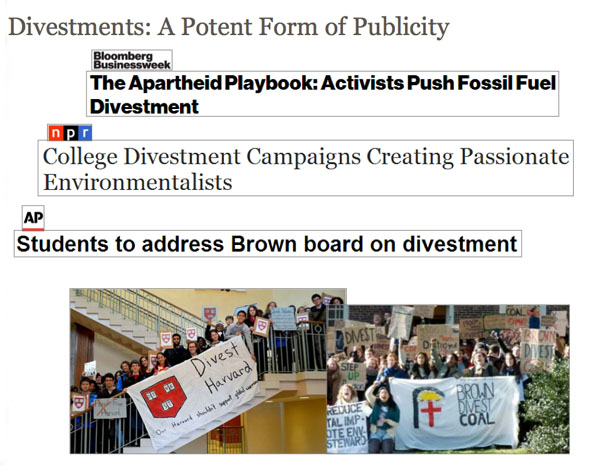
\includegraphics[width=100mm]{s7-divest-slide.png}
\centering
\caption{One slide from the slideshow on threats to the coal industry. Source: Meredith Xcelerated Marketing}
\label{fig:DivestSlide}
\end{figure}




Divestment would signal that the `smart money' is shifting away from fossil fuels. 
This could help produce a political climate in which significant action can be taken, including in the form of carbon pricing and reduced subsidies for fossil fuels.\footnote{See also: ``Companies like ExxonMobil, Shell, BP have billions of dollars/euros. How can divesting the funds from a few institutions like universities, pensions and churches make an impact?'' at: \url{http://gofossilfree.org/faq/}}


	
	\subsection{What are the University of Toronto's peer schools doing?}
	\label{PeerSchools}



Fossil fuel divestment campaigns are active at more than 300 schools across North America, including:
\begin{itemize}
	\item Harvard, Yale, Princeton, Stanford, MIT, Duke, Caltech, the University of Michigan, Tufts, Wellesley,
	\item The University of British Columbia, McGill, the University of New Brunswick--Fredericton, the University of Victoria, McMaster University, Concordia University, Simon Fraser University,
	\item and Oxford University.
\end{itemize}
To date, six universities and colleges have pledged to pursue fossil fuel divestment : San Francisco State University Foundation, Hampshire College, Unity College, Sterling College, College of the Atlantic, and Green Mountain College.\footnote{For a complete and up-to-date list, see: \url{http://campaigns.gofossilfree.org/}}



Divestment campaigns are active at many prominent American schools:
\begin{itemize}
	\item Divest \textbf{Harvard} has met with the university administration and with trustees to discuss divestment.\footcite[][]{HarvardMeeting} \footcite[][]{HarvardTrustees} On April 11th 2013, 1,300 petition signatures were delivered to the Harvard administration in support of divestment.\footcite[][]{HarvardPetition} 71 percent of students supported a referendum calling for fossil fuel divestment.\footcite[][]{StudentsClamoring}
	\item On May 30th 2013, the faculty senate at the \textbf{University of California}, Santa Barbara voted in favour of fossil fuel divestment. Earlier that week, the student government at Stanford University voted in favour of divestment. In total, the student governments at seven campuses of the University of California have voted in favour of divestment.\footcite[][]{UCSB2013}
	\item At \textbf{Stanford}, the undergraduate senate passed a resolution in support of fossil fuel divestment in May 2013.\footcite[][]{StanfordSenate}
	\item The president of \textbf{Tufts University} has established a working committee to consider fossil fuel divestment, as well as other steps the school could take to address climate change.\footcite[][]{TuftsDivest}
	\item \textbf{Hampshire College}, which was the first university to divest from South Africa during the 1980s, was also the first school to officially commit to fossil fuel divestment.\footcite[][]{StudentsClamoring}
\end{itemize}



Divestment is also being considered at schools across Canada:
\begin{itemize}
	\item The \textbf{McGill} divestment campaign is the most advanced of the Canadian divestment campaigns: the three major student unions have endorsed the divestment campaign, the petition was presented to the Board of Governors on February 1st, and was rejected on by the Board of Governors on May 23rd 2013.\footcite[][]{McGillStudentExecs} \footcite[][]{McGillDelivers}
	\item At the \textbf{University of New Brunswick}, students have collected over 300 signatures in support of divestment.\footcite[][]{UNBPetition} They have also submitted a presentation and resolution of support to the student union.\footcite[][]{UNBStudentUnion}
	\item At the \textbf{University of British Columbia}, students are calling on the UBC Investment Management Trust to sell the school's \$7.14 million in oil and gas investments.\footcite[][]{UBCDivest} In June 2013, UBC adopted a new responsible investment strategy.
\end{itemize}



No major university has yet committed to divest from fossil fuels.
This gives the University of Toronto an opportunity to distinguish itself and show leadership.
As the severity of climate change worsens, the case for divestment will strengthen; at the same time, as governments become more active it will become increasingly clear that fossil fuel stocks are overvalued.
By moving early, the University of Toronto can contain this risk and gain reputational advantages.



\subsubsection{Questions about divestment raised at other schools}



At other universities where fossil fuel divestment has been proposed, university administrations have responded with specific objections about the proposed course of action.
Toronto350.org's fossil fuel divestment proposal has been designed to take these considerations into account and this brief includes detailed responses to a number of counter-arguments.



At McGill, a proposal to divest from oil sands and fossil fuels was considered and rejected by the university administration in May 2013.\footnote{The proposal is available at: \url{http://Toronto350.org/brief/mcgill/the-social-injury-of-tar-sands-and-fossil-fuels.pdf} and the response is at: \url{http://Toronto350.org/brief/mcgill/camsr_documents_0.pdf}}
The issues raised by the McGill administration are addressed comprehensively in this brief.
For instance, the Report of the Committee to Advise on Matters of Social Responsibility states that:
\begin{quote}
In discussion with the Committee, the representatives of Divest McGill acknowledged they were unaware of examples of corporations involved in oil sands and fossil fuels which had been found to have violated or frustrated the enforcement of rules of domestic or international law intended to protect individuals against deprivation of health, safety or basic freedoms.\footcite[][p. 4]{McGillRejection}
\end{quote}
Two sections of this brief address this matter: \nameref{sec:FrustrateLaw} and \nameref{LegalPrecedents}



McGill's Committee to Advise on Matters of Social Responsibility also states that:
\begin{quote}
During the discussion, it was noted that a number of energy companies are actively engaged in research into and the production of alternate forms of energy, which suggests that investment in these companies may help to promote and encourage the use of alternate sources of energy.\footcite[][p. 4]{McGillRejection}
\end{quote}
This specific objection is addressed in: \nameref{RenewableInvest}



The committee at McGill also ``took note that the energy sector, including oil and gas extraction, production and distribution, is highly regulated by government at all levels''. This objection is considered in the section: \nameref{HeavilyRegulated}



In conclusion, the committee at McGill decided that:
\begin{quote}
While some members noted environmental and health effects related to the oil sands, the Committee found that Divest McGill had presented no evidence of a court finding of injury on the part of oil sands or fossil fuels companies, and otherwise had provided insufficient data and evidence to establish that social injury had occurred.\footcite[][p. 4]{McGillRejection}
\end{quote}
This brief provides detailed evidence of the social injury caused by fossil fuel companies, in the section: \nameref{sec:SocialInjury}.



Divestment as proposed by Toronto350.org is substantially more focused than what was presented by Divest McGill.
This proposal calls only for the sale of direct holdings in 200 listed companies, and does not call upon the university to identify firms involved in any specific fossil fuel related activity.
Furthermore, this proposal does not call for divestment from companies that make loans to the 200 companies listed.
This greatly simplifies the process of divestment, and removes any uncertainty about whether the firms in question are directly involved in the social injury described in this brief.



On June 4th 2013, the Board of Governors of the University of British Columbia (UBC) approved a new responsible investment strategy that included a number of objections to using divestment in response to concern about companies causing social injury.\footcite[][]{UBCRespInv}



The first concern raised is about the challenge of effectively screening potential investments according to environmental, social, and governance concerns:
\begin{quote}
Issues with portfolio screening are multiple and complex. Ethically, portfolio screening is difficult to apply to reflect the competing political, environmental and social interests playing out at any given time, and whether these interests should be company specific or sector-wide.
\end{quote}
This concern is eliminated in the approach proposed at the University of Toronto.
The list of companies where divestment is encouraged is already prepared and included in: \nameref{sec:200Companies}.
Since these are the 200 global companies with the largest fossil fuel reserves, there is a direct logical reason why they each is included in the list.
This pertains both to the degree of social injury that would be caused by the burning of their reserves, as well as the degree of regulatory risk involved in investing in these firms, given the growing willingness of governments to regulate GHG pollution.



Another issue raised in the UBC document is:
\begin{quote}
Economically, screening out entire sectors such as the Canadian energy sector would push more of the endowment outside of the country, into geographic areas that often have more questionable social and environmental records.
\end{quote}
The 200 companies listed in this proposal are global, mitigating the risk that U of T would shift its endowment into more damaging companies elsewhere.
This brief also includes a response to the concern: \nameref{CanadianJobsEconomy}



The last objection to divestment included in the UBC document is:
\begin{quote}
Financially, implementing a direct screening policy would prevent UBC from investing in pooled or indexed funds and would generate significant overhead that would negatively impact student and researchers supported by the endowment.
\end{quote}
Once again, this concern does not apply to the approach proposed by Toronto350.org, which calls only for divestment of direct stock holdings at this time.



	\subsection{What are other large investors doing?}
	\label{LargeInvestors}



Several cities are considering divesting themselves from fossil fuel stocks.\footnote{See: \url{http://gofossilfree.org/commitments/}}
The mayor of Seattle has called for the city to divest its fund for daily operations (US\$1.4 billion), its deferred compensation plan (US\$700 million), and its pension system (US\$1.9 billion).\footcite[][]{SeattleDivest}
The mayor of Portland, Oregon has urged the Oregon State Treasurer, the Local Government Investment Pool, and the Oregon Investment Council to divest all state holdings in fossil fuel companies.
The San Francisco Board of Supervisors has urged the retirement board to divest US\$583 million of fossil fuel holdings in the city's \$16 billion retirement fund.\footcite[][]{DivestProtect40to60}
In June 2013, the city council of Providence, Rhode Island voted 11-1 in favour of divestment.\footcite[][]{ProvidenceDivest}



Eleven regional conferences of the United Church of Christ in the United States have voted to divest.\footcite[][]{ChurchesFFDivestment}
Numerous other churches and faith-based organizations are considering divestment, including the First Unitarian Church of Salt Lake City, the Evangelical Lutheran Church of Oregon, and the Uniting Church of New South Wales \& ACT, Australia.



Hedge fund billionaire Tom Steyer has decided to divest his holdings in fossil fuel companies.
He thinks that a portfolio that excludes fossil fuels ``will outperform the market''.\footcite[][]{SteyerMiddleburyLetter}
In July 2013, the Norwegian financial services company Storebrand ASA announced that they will be divesting from 19 fossil fuel companies.\footcite[][]{StorebrandPR}
The decision was motivated by the belief that the value of these companies would fall because of their negative climate change impacts.\footcite[][]{StorebrandNews} \footcite[See also: ][]{GristStorebrand}
The Dutch bank Rabobank has also decided not to fund shale oil development.\footcite[][]{RabobankRefuses}
According to a spokesperson from the bank, this is because ``[t]he bank's global policy is not to be involved with extracting fossil fuels where it is not clear what the risks and consequences may be''.\footcite[][]{RabobankNews}



In July 2013, European Union Climate Commissioner Connie Hedegaard called for the European Investment Bank (EIB), the European Bank for Reconstruction and Development (EBRD), and the World Bank to eliminate public support for fossil fuels.\footcite[][p. 9--10]{InvestHasteRepent} \footcite[See also:][]{HedegaardAppeal}
Each year, these three institutions provide US\$168 billion in funding for projects around the world.\footcite[][p. 10]{InvestHasteRepent}


	
	\subsection{But don't fossil fuel companies also invest in renewable energy?}
	\label{RenewableInvest}



In 2008, British Petroleum (BP) launched a rebranding effort in which it claimed that its initials now meant `Beyond Petroleum'.\footcite[][]{GreenwashBP}
This is now widely seen as an example of `greenwashing' --- a practice defined as devoting extensive resources to advertising how environmentally-friendly an organization claims to be, while not actually adopting sustainable practices.\footnote{The Oxford English Dictionary defines the term as: ``The creation or propagation of an unfounded or misleading environmentalist image''}
BP has since abandoned its foray into solar power generation and put its U.S. wind-farm business up for sale.\footcite[][]{BPNoLongerBeyond} \footcite[][]{BPNoMore}
This behavious is typical of the fossil fuel industry, which has spent vast sums of money touting its environmental credentials, at the same time as their business plans --- which depend on burning all of their fossil fuel reserves --- are fundamentally at odds with environmental sustainability.
As BP's chief executive, John Browne spent \$200 million advertising the `Beyond Petroleum' slogan.
Under his tenure, BP was ``marred by a succession of devastating accidents... [including] an explosion at BP's Texas City refinery in 2005 that killed 15 workers and injured 170 others, and an oil spill a year later that dumped 4,800 barrels of oil at Prudhoe Bay, on the coast of Alaska''.\footcite[][]{BlackStuffBP}
In April 2010, BP's Deepwater Horizon oil platform in the Gulf of Mexico exploded, causing over \$40 billion in damage, alongside massive ecological harm.\footcite[][]{OffshoreLiability}
All told, BP may end up paying over US\$90 billion in fines and compensation for causing the disaster.\footcite[][p. 20]{Supermajordammerung}
At the peak, BP was directing 6 percent of overall investment toward renewables.
This compares with 2.5 percent at Chevron and Shell, with no other major oil company investing more than 1 percent.\footcite[][]{RSBigOilLies}



The sums being invested in renewable energy by fossil fuel companies are dwarfed by the investments they are making in unconventional sources of coal, oil, and gas.
For example, BP has announced its intention to increase spending on arctic drilling by \$1 billion over five years, increasing its fleet of oil rigs from seven to nine by 2016.\footcite[][]{BPArcticBillion}
In 2003, BP invested \$6.75 billion in Russia's Tyumen Oil Company, which is involved with the massive Sakhalin offshore project.\footcite[][]{NotBeyondInRussia}
In total, the Government of Alberta expects over \$218 billion to be invested in the oil sands over the next 25 years.\footcite[][]{OilSandsEconBenef}
The 200 fossil fuel companies with the largest reserves spent \$674 billion in 2012 identifying and developing new fossil fuel reserves, as well as researching ways to extract fossil fuels from proven reserves.\footcite[][p. 4]{CTI2012} \footcite[See also: ][]{SteinerFinancialSector}



Conventional fossil fuel sources are more than sufficiently abundant to allow humanity to far exceed the 2˚C `safe limit' for climate change.
The costly pursuit of exotic new reserves shows how fossil fuel companies have failed to internalize the reality of climate change and are continuing to implement investment plans that are sharply at odds with planetary safety.
Also, based on various credible estimates of the social cost of carbon, the total damage being done to society by fossil fuel burning substantially exceeds the scale of the investments the industry is making in renewables.\footnote{See: \nameref{sec:PricingSocialCost}}

	
	
	\subsection{In what cases have courts found that fossil fuel companies caused injury?}
	\label{LegalPrecedents}
	
	
	
So far, there are a limited number of legal precedents in which the seriousness of climate change and the injury being caused by fossil fuel companies are recognized.
Those that exist can be found in: \nameref{sec:FrustrateLaw}.
The Supreme Court of British Columbia decision ``Tsilhqot'in Nation v. British Columbia'' acknowledges climate change impacts on mountain pine beetles, and on biodiversity generally.\footcite[][p. 358, 406]{Tsilhqotin}


In past instances, the University of Toronto has accepted the appropriateness of divestment before a comprehensive legal justification has been in place.


\begin{vcom}
Find information about how U of T divested from South Africa before Canada passed the law to facilitate that. Also, the tobacco precedent.
\end{vcom}


\begin{vcom}
* Legal efforts by small island states
* One example: https://www.sindark.com/2008/09/14/carbon-emissions-worse-than-criminal-damage/
* Fossil fuel companies also cause injury in forms other than climate
* Oil spills - Deepwater Horizon
* Toxic air pollution - deaths from coal
* This guy might be able to make some suggestions: http://www.law.columbia.edu/courses/L8451-advanced-climate-change-law/spring-2013/section-001
* Also: http://envirolaw.com/about/meet-dianne/
\end{vcom}
	
	
	
	\subsection{Isn't the energy sector, including oil and gas extraction, production and distribution, highly regulated by government at all levels?}
	\label{HeavilyRegulated}
	


When it comes to GHG pollution, the fossil fuel industry is essentially unregulated at the federal level in Canada.
Firms are free to use the atmosphere as a dumping ground for \ce{CO2} pollution.\footcite[See: ][]{Paris2013} \footcite[See also: ][]{Stewart2013}
The harm the industry is causing is largely dispersed, which makes it hard to assign responsibility, but we know there are major damaging impacts in the aggregate.



Not only that, but many governments in Canada have adopted policies intended to accelerate the growth of the fossil fuel sector.
These include aggressive international lobbying for oil pipelines and other forms of fossil fuel export infrastructure.\footcite[See, for example: ][]{KeystoneLobbyingHarder} \footcite[][]{HarperNoBrainer} \footcite[][]{OliverRadicalLetter}
They also include steps to weaken environmental assessment processes, reduce the scope of scientific research being conducted on climate change while suppressing the publication of results from government scientists, and substantial continuing subsidies to the fossil fuel industry.



The regulation that exists in Canada is not putting the country on a pathway toward making a fair contribution in the global climate change mitigation effort.
Additional regulation is required and --- until it is in place --- socially conscious organizations should take action themselves in response to the harm being caused by fossil fuels.


	
	\subsection{Can humanity manage without fossil fuels?}
	\label{DoingWithout}



This question was extensively examined by Cambridge physicist David MacKay, resulting in his 2009 book \emph{Sustainable Energy – without the hot air}, which is available for free online.\footcite[][]{MacKay2009}
In his detailed analysis, MacKay considers both the scope for reducing energy demand through energy efficiency and the opportunities for producing energy from low- and zero-carbon sources like renewables and nuclear power.
In order to demonstrate the feasibility of providing everyone in the world with enough energy to sustain a high standard of living, MacKay calculates that ``[t]o supply every person in the world with an average European's power consumption (125 kWh/d [kilowatt-hours per day]), the area required would be two 1000 km by 1000 km squares in the desert''.\footcite[][p. 178]{MacKay2009}
Although doing this with only giant solar facilities would be impractical and probably expensive, the example nonetheless demonstrates that humanity can enjoy an improved standard of living without relying on fossil fuels at all.
MacKay concludes that by combining wind, hydro, tidal, wave, geothermal, solar, and nuclear power it is possible for everyone in the world to consume 80 kWh per day --- equivalent to the total per capita energy use in Hong Kong today.\footcite[][p. 106, 238]{MacKay2009}



The opportunities associated with renewable energy deployment are already being realized, and major growth potential remains.
The U.S. Department of Energy believes that by 2030, 20 percent of American electricity could come from wind, reducing annual electric sector \ce{CO2} emissions by 825 million metric tons.\footcite[][]{20PercentBy2030}
Iowa already generates 39 percent of its energy from this low-carbon source.\footcite[][]{BlownAway}
Concerns about the intermittency of wind energy have also proven exaggerated; by balancing production from wind facilities in different areas, consistent power output can be created.\footcite[][]{BlownAway}



Huge opportunities exist to reduce energy use by improving efficiency, including in industry, transport, power generation, and buildings.
According to the International Energy Agency (IEA), these possibilities have not yet been factored into government planning: ``[t]wo-thirds of the economic potential to improve energy efficiency remains untapped in the period to 2035'' and energy efficiency remains ``a huge opportunity going unrealised''.\footcite[][p. 13]{IEA2012press}
The IEA explains that ``[e]conomically viable efficiency measures can halve energy demand growth to 2035'' and produce reductions in oil use equivalent to the production from Russia and Norway.\footcite[][p. 14]{IEA2012press}
By 2035, the IEA predicts that improved energy efficiency could cut energy expenditures by 20 percent, alongside ``wider economic gains, particularly for India, China, the United States and Europe''.\footcite[][p. 15]{IEA2012press}



The transition to renewable energy will bring jobs and other economic benefits.
Analysis from the Union of Concerned Scientists found that a national standard of 25 percent renewable energy in the United States by 2025 would ``create more `green' jobs, lower consumer energy bills in every region of the country, and reduce carbon dioxide (\ce{CO2}) and other harmful emissions from power plants—the biggest source of global warming pollution in the United States.''\footcite[][]{ConcernedScientistsJobs}
The report finds that this policy would create three times as many jobs as producing the same amount of energy from fossil fuels.\footcite[See also: ][]{CSBenefitsRenewable}
A zero-carbon energy system would also reduce volatility in energy prices, since the inputs are free once the infrastructure is built, and would eliminate the security and economic risks experienced by states dependent on fossil fuel imports.



On a business-as-usual pathway in which humanity burns most or all of the planet's remaining fossil fuels, the planet can be expected to experience catastrophic changes that will wreak considerable economic damage.
As such, the choice we are facing is not between perpetuating the \emph{status quo} indefinitely or committing to decarbonization.
Rather, our choice is between decarbonization and catastrophic climate change.
The World Bank has argued that ``[t]he current level of action puts us on a pathway towards a 3.5–4°C warmer world by the end of this century'' and that ``[s]uch a scenario would have a devastating impact on the climate and would threaten our current economic model with unprecedented and unpredictable impacts on human life and ecosystems in the long term.''\footcite[][p. 13]{WorldBankCarbonPricing} \footcite[See also:][]{WoesReverse}
As the Australian government's Climate Commission explains: ``Burning all fossil fuel reserves would lead to unprecedented changes in climate so severe that they will challenge the existence of our society as we know it today.''\footcite[][p. 5]{CriticalDecade2013}


Whether we like it or not, humanity must learn how to manage without fossil fuels.



	\subsection{Won't divestment hurt the endowment, including U of T's ability to provide scholarships?}
	\label{HurtEndowment}
	
	
	
As discussed at greater length in \nameref{NoDivestPenalty}, there is evidence that portfolios that exclude companies that cause social injury do not suffer a financial penalty for doing so.
Deutsche Bank and Mercer have conducted major meta-studies on portfolios that consider environmental, social and governance (ESG) factors and found that there is either a neutral or positive relationships between financial performance and the incorporation of ESG factors into portfolio management.\footcite{DeutscheBankSI} \footcite{MercerRI}
Hedge fund billionaire Tom Steyer explains in a letter to the Corporation of Brown University:
\begin{quote}
The available research, looking backward, shows that the return penalty would be tiny—but in any event good investors rarely look backward. Looking to the future, the data on climate change makes it clear that something has changed, and as the rest of the world realizes this, coal stocks will come under increasing pressure. At the moment, other investors have not fully realized the risk that carbon reserves will become a stranded asset; if you acknowledge what your own science departments are telling you this gives you an edge relative to those investors. I can tell you that in my own investments, I have directed my financial team to divest my holdings of coal investments so that I will have a coal free portfolio myself – in part because I am convinced it will outperform the market.\footcite[][]{SteyerBrownLetter} \footcite[See also: ][]{SteyerMiddleburyLetter}
\end{quote}
Unlike fossil fuel divestment, failing to deal with the `carbon bubble' could harm the university's financial standing in the long term.



Universities are entities that expect to exist forever and which therefore have very long time horizons for their investment decisions.
In the long term, the university's ability to fund research and provide scholarships depends on general financial health, which would be improved by divestment.




	\subsection{Won't fossil fuel companies stop making donations to U of T?}
	\label{NoMoreDonations}



Donations from fossil fuel companies are reasonably limited. 
For instance, `President's Circle' donors who have given over \$1,827 annually include Husky Energy, the Imperial Oil Foundation, the Mitsui Canada Foundation, Petro-Canada (a subsidiary of Suncor), RioTinto Alcan, and Shell Canada.\footnote{See: \url{http://boundless.utoronto.ca/member-listing/}}
The full list includes several hundred donors.
Three fossil fuel companies have also participated in the university's Boundless campaign: Husky Energy Inc., RioTinto Alcan, and the Mitsui Canada Foundation.\footnote{See: \url{http://boundless.utoronto.ca/member-listing/}}
Once again, the list includes a dominant share of non-fossil-fuel-corporation donors.



These donations do not offset the financial risks associated with heavy investment in fossil fuels, nor do they compensate for the ways in which fossil fuel investments are contrary to the university's values and policies.



Two major motivations for corporate donations to the university are advertising and positive publicity.
Neither of these objectives would be undermined by divestment, so it is plausible that corporate donations from fossil fuel companies could continue in spite of divestment.



When Unity College divested, they experienced an uptick in applications and donations.\footcite[][p. 4]{CaseForDivestment}



	\subsection{Shouldn't U of T fight climate change through research and education?}
	\label{ResearchEducation}



U of T is active in climate change research and teaching, and this will continue.\footnote{See: \nameref{UofTAcademicProgramming}}
This research has helped to establish what a serious and pressing problem climate change is for people in Canada and around the world.
Although this work is very welcome, it is not a substitute for divestment.
The very existence of the divestment policy shows that the university has accepted the basic argument that some investments can be incompatible with the values of the university.



	\subsection{Won't divestment hurt Canadian jobs and the economy?}
	\label{CanadianJobsEconomy}
	
	

This question gets the argument backwards: not dealing with climate change could cause enormous harm to Canadian prosperity.
At the same time, there are major risks associated with continuing to invest hugely in fossil fuel infrastructure, at a time when the policy-makers of the world are starting to get serious about controlling climate change.
As detailed extensively in section 3 (\nameref{sec:SocialInjury}), climate change poses a serious risk to Canadian prosperity. 
Furthermore, as detailed in section 4 (\nameref{sec:Fiduciary}), there are major risks associated with continuing to invest in fossil fuel projects.


Right now, the Canadian economy is excessively dependent on fossil fuel production and export.
Canada also has excessively high \emph{per-capita} emissions of GHG pollution - meaning we will probably need to cut faster and deeper than most, as part of a fair global transition to a low-carbon economy.
Given that the future will be carbon-constrained, it is urgent that we start mitigating that dependence.
Divestment by the University of Toronto would send an important signal to help initiate this necessary transition.
As highlighted in the Stern Review: ``The benefits of strong, early action on climate change outweigh the costs''.\footcite[][p. i]{Stern2007}
Early divestment could also help reduce the risk of large amounts of investment being tied up in fossil fuel projects that will need to be shut down before the end of their economic lives as global and Canadian restrictions on GHG pollution are tightened.



Furthermore, as the world gets serious about decarbonization, extensive economic opportunities will arise in this sector.
These will include the retrofitting of buildings to improve efficiency, the construction of renewable energy infrastructure, and research and development to support and enhance the transition.
As a key research institution, U of T can participate directly in that part of the world's economic realignment.



	\subsection{Can't we just adapt to climate change?}
	\label{WhyNotAdapt}



As described at considerable length in section 3 (\nameref{sec:SocialInjury}), the impacts of even 2˚C of climate change would be severe, and a business-as-usual pathway in which we continue to use fossil fuels the way we do now would likely see temperatures up more than 5˚C by 2100.


There is no adapting to climate change that melts the Greenland and West Antarctic ice sheets, flooding huge populated areas.
Similarly, climate change on such a scale would be accompanied by an acute risk of abrupt and irreversible effects.
In order to have a reasonable chance of adaption that leads to a world with comparable human prosperity to what we enjoy now, climate change must be kept under 2˚C.
That means most of the world's fossil fuels cannot be burned, leading to the various implications described in this brief.



	\subsection{Won't carbon capture and storage (CCS) save us?}
	\label{CCSSaves}



Carbon capture and storage (also called carbon capture and sequestration) is a technology that promises to separate \ce{CO2} from the emissions of facilities like power plants and bury it in underground formations such as saline aquifers.
The technology has already been deployed in certain applications, such as the re-injection of unwanted \ce{CO2} Sleipner gasfield in Norway.



CCS cannot solve our climate change problem for two major reasons: scale and economics.



Humanity is now emitting roughly 30 billion tonnes of \ce{CO2} into the atmosphere annually.\footcite[][]{RedrawingClimateEnergy}
As explained in an article in the \emph{MIT Technology Review}: ``[I]f we were to bury just one-fifth of the global carbon dioxide emissions, we would need to build an industry capable of handling twice the volume of stuff as the entire oil industry, an industry that took 100 years to develop, driven by a large and mostly expanding market.''\footcite[][]{BullisonCCS}
Rather than being a genuine means for dealing with climate change, CCS has more often been a way for the fossil fuel industry to delay serious government action by claiming that a wonderful technological solution will soon exist.
This claim is at odds with the difficulties encountered by test projects like FutureGen --- a supposedly `clean' coal-fired power plant announced by President George W. Bush in 2003, but which was subsequently scrapped because of intolerably high costs.
As \emph{The Economist} explains: ``there is not a single big power plant using CCS anywhere in the world''.\footcite[][]{TroubleInStore}



On the economics of CCS, \emph{The Economist} explains:
\begin{quote}
The problem with CCS is the cost. The chemical steps in the capture consume energy, as do the compression and transport of the carbon dioxide. That will use up a quarter or more of the output of a power station fitted with CCS, according to most estimates. So plants with CCS will need to be at least a third bigger than normal ones to generate the same net amount of power, and will also consume at least a third more fuel. In addition, there is the extra expense of building the capture plant and the injection pipelines. If the storage site is far from the power plant, yet more energy will be needed to move the carbon dioxide.\footcite[][]{TroubleInStore}
\end{quote}
Despite considerable government subsidies, including \$3.4 billion in an Americans stimulus bill, CCS remains unattractive to energy utilities largely because of cost.\footcite[][]{IllusionCleanCoal}
In a discussion paper published by the Belfer Center for Science and International Affairs at Harvard, it was estimated that sequestering one tonne of \ce{CO2} would cost approximately \$150 --- far more than the cost of avoiding the emissions in the first place by implementing lower-cost measures.\footcite[][]{RealisticCostsCarbonCapture}



Other considerations include the stability of formations into which \ce{CO2} is injected and the seismic consequences of doing so.\footcite[][]{CCSEarthquake} \footcite[See also: ][]{AFPonCCS}
Carbon dioxide is heavier than air, so leaks from CCS facilities could smother people and animals nearby.\footcite[][]{TroubleInStore}
Water saturated with \ce{CO2} also becomes acidic, which could undermine the integrity of equipment and underground formations intended to contain it.
CCS is also useless for mobile sources of emissions where \ce{CO2} cannot plausibly be separated from waste gases and stored.
Given that 85 percent of the total emissions associated with fuels from the oil sands occur when the fuels are burned in vehicles, this means the scope for decreasing the climate impact of the oil sands with CCS is especially limited.\footcite[][]{HardToScrub} \footcite[][]{NoSilverBullet}



The failure of CCS to live up to its promise is especially problematic for Canada, given the degree to which the climate change plans of the federal government and the Government of Alberta depend on this technology becoming cheap and effective in the near term.
Canada's unrealistic expectations for CCS mean that decarbonization will be even more challenging than expected by the federal and provincial governments, making it all the more important to begin investing in decarbonization now.



	\subsection{Won't geoengineering save us?}
	\label{GeoSaves}
	
	
Geoengineering is the deliberate modification of the climate system, intended to counteract the effect of anthropogenic climate change.
Several different mechanisms for achieving this have been proposed, but all are deeply problematic for a variety of reasons.
Geoengineering mechanisms can be broadly broken down into those that would seek to reduce global temperatures without lowering atmospheric \ce{CO2} concentrations and those that would actually seek to draw \ce{CO2} from the atmosphere.



The latter sort --- which could theoretically reduce the atmospheric concentration of GHGs --- suffer from the same problems of scale and economics experienced by CCS, exacerbated by the additional cost of separating \ce{CO2} from air (where it is relatively low in concentration) rather than directly from the waste stream of power plants and other facilities where it is relatively concentrated.  



The former sort, which could be achieved through means like injecting large volumes of sulfate aerosols into the upper atmosphere, suffers from even more significant problems.
For one thing, it would do nothing to stop the acidification of the world's oceans: a trend that threatens to destroy the ability of marine organisms to form shells and skeletons from calcium, along with other unknown global effects on marine food webs.
For another, geoengineering of this type would be likely to further alter global precipitation patterns, in addition to the changes that would be created by climate change.
This sort of intervention would also need to be undertaken constantly and forever; if it were to be discontinued, global temperatures would spike.



In short, geoengineering adds new risks on top of those from climate change, there is no guarantee it would be effective in reducing global temperatures and addressing the other consequences of climate change, and it would be likely to bring significant side-effects.
Choosing to geoengineer would mean choosing to impose even more risk and damage upon future generations than we already are.



% END SECTION 7